%%%%%%%%%%%% Attribution %%%%%%%%%%%%
% This template was created by 
% Chuck F. Rocca at WCSU and may be
% copied and used freely for 
% non-commercial purposes.
% 10-17-2021
%%%%%%%%%%%%%%%%%%%%%%%%%%%%%%%%%%%%%

%%%%%%% Start Document Header %%%%%%%
% In creating a new document
% copy and paste the header 
% as is.
%%%%%%%%%%%%%%%%%%%%%%%%%%%%%%%%%%%%%

\documentclass[12pt]{article}

%%%% Header Information %%%%
    %%% Document Settings %%%%
    \usepackage[utf8]{inputenc}
    \usepackage[
        twoside,
        top=1in,
        bottom=0.75in,
        inner=0.5in,
        outer=0.5in
    ]{geometry}
    \pagestyle{myheadings}

%%%% Additional Commands to Load %%%%
    \usepackage{tcolorbox}
    \tcbuselibrary{skins}
    \usepackage{minted}
    \usepackage{color}
    \usepackage{tikz}
    \usetikzlibrary{calc}
    \usepackage{tabularx,colortbl}
    \usepackage{amsfonts,amsmath,amssymb}
    \usepackage{titling}
    \usepackage{mathrsfs}
    \usepackage{calc}
    \usepackage{graphicx}
    \graphicspath{ {./images/} }
    \usepackage{tabularx}

%%%% Commands to Define Homework Boxes %%%%
%%%% Box Definition %%%%
    \newtcolorbox{prob}[1]{
    % Set box style
     %   sidebyside,
     %   sidebyside align=top,
    % Dimensions and layout
        width=\textwidth,
        toptitle=2.5pt,
        bottomtitle=2.5pt,
        righthand width=0.25\textwidth,
    % Coloring
        colbacktitle=gray!30,
        coltitle=black,
        colback=white,
        colframe=black,
    % Title formatting
        title={
            #1 \hfill \phantom{WWWW}
        },
        fonttitle=\large\bfseries
    }

%%%% Environment Definition %%%%
    \newenvironment{problem}[2][Problem]
    {
        \begin{prob}{#1}
    }
    {
        \tcblower
        \centering
        \textit{\scriptsize\bfseries Working out}
        \vspace{{#2}}
        \end{prob}
    }



%%%% Document Information %%%%
    \title{Welcome!}
    \author{Prime Time}
    \date{Februrary \(8^{th}\) 2024}

%%%%%%% End Document Header %%%%%%%


%%%% Begin Document %%%%
% note that the document starts with
% \begin{document} and ends with
% \end{document}
%%%%%%%%%%%%%%%%%%%%%%%%

\begin{document}

%%%% Format Running Header %%%%%
\markboth{\theauthor}{\thetitle}

%%%% Insert the Title Information %%%
\maketitle


%%%% General Description of the Document %%%%
\begin{abstract}
    \begin{center}
        Welcome along to the first meeting of Prime Time!
    \end{center}
    This is a club where we look at the fun an interesting topics in mathematics. All students from all grades are welcome to attend. Each week you will be introduced to a concept or a problem in mathematics, these are meant to challenge you, the following week we will share and discuss our solutions. 
\end{abstract}


%%%% Introduction to the General Template %%%%
\section{Ready!}
    Each week we will get ready with some smaller maths puzzles.
    Today we will get started with some patterns.

    \begin{problem}{Continue the pattern then write the rule}{8cm}
        \vspace{5mm}
        a. 1, 2, 4, 8, 16, 32, ..., % Geometric Sequence i,e (Common Ratio) of *2; Next number is 64
        \vspace{0.5cm}

        b. 1, 4, 7, 10, 13, 16, ..., % Arithmetic Sequence i.e (Common Difference) of +3; Next number is 19
        \vspace{0.5cm}

        c. 1, 3, 6, 10, 15, 21, ..., % The Triangular Numbers Numbers that can be arranged in to a triangular shape; Next number is 28
        \vspace{0.5cm}
    \end{problem}

\section{Set!}
    \begin{problem}{Moser's Circle Problem}
     Below are several circles with n points on circles for n = 2, 3, 4, 5 and chords (line segments whose endpoints are on the circle) connecting the points. The points on the circle are chosen such that no three chords intersect at a single point inside the circle.\\
    
        \begin{center}
            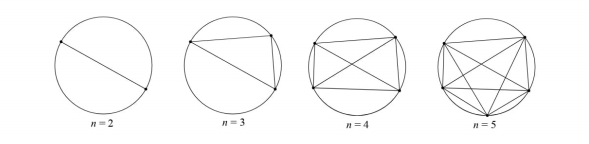
\includegraphics[width=0.8\textwidth]{images/Mosers-Circle-Problem.png}
        \end{center}
     
     a. Count the number of non-overlapping regions created by the chords.
     
     b. Complete the table.
     \begin{center}
\begin{tabularx}{0.8\textwidth} { 
  | >{\hsize=.4\textwidth\raggedleft\arraybackslash}X|| >{\centering\arraybackslash}X | >{\centering\arraybackslash}X | >{\centering\arraybackslash}X | >{\centering\arraybackslash}X | }
 \hline
 $n$, number of points & 2 & 3 & 4 & 5 \\
 \hline
 number of non-overlapping regions  & 2  & 4 &  &  \\
\hline
\end{tabularx}
\end{center}
c. What is the rule for the sequence? \emph{Write your answer in terms of $n$}

d. Predict the next number in the sequence.
    \end{problem}
\section{Go!}

\end{document}
